\chapter{Conclusiones}

\section{Resultados}

Durante todo el periodo de desarrollo del proyecto se ha conseguido implementar la arquitectura definida en el capítulo de Desarrollo. Se ha conseguido cumplir el objetivo
de diseñar e implementar una arquitectura robusta y que ha conseguido gestionar la información proveninente de la API de Twitter y guardarla en la base de datos de forma
satisfactoria.

Otro de los objetivos conseguidos, ha sido conocer el uso de las APIs de Google Maps y Twitter a fondo para luego poder aplicarlas correctamente
en la aplicación.

Respecto a los requisitos definidos, se han podido implementar la mayoría de los requisitos exceptuando \textbf{FS-U-01},\textbf{FB-A-03}. Para el caso de la valoracion de las
entradas del blog(\textbf{FS-U-01}) se ha dejado para el siguiente sprint debido a ser una funcionalidad no básica de la aplicación. Para el requisito \textbf{FB-A-03}
de mostrar los comentarios asociados a la entrada del blog se ha tenido que posponer para un siguiente sprint, debido a los requisitos \textbf{FB-U-04} y \textbf{FB-A-05} correspondientes
al mapa de Tweets y su parte de administración han supuesto realizar mas iteraciones de las previstas. Para el caso \textbf{FB-A-03} de gestionar el contenido de la entrada, se ha
podido completar pero con la existencia de un fallo a la hora de subir imágenes.


Con la parte de maquetación finalizada, se lleva acabo un testeo y prueba de la aplicación en los distintos navegadores web. Se realizan testeos con los siguientes
navegadores:

\begin{itemize}
\item Google Chrome, Mozilla Firefox para los sistemas operativos de Android,IOS,Windows y Mac OS.
\item Safari para IOS y Mac OS.
\item Internet Explorer 11 para Windows.
\end{itemize}

El testeo en estos navegadores ha sido satisfactorio y responde adecuadamente a los estilos aplicados y cambios de resolución aplicados mediante CSS.

En definitiva, se podría decir que se ha conseguido el objetivo principal de desarrollar un proyecto que funciona como herramienta orientada a marketing y
como un portal de promoción de la gastronomía. Esta versión de la aplicación proporcionará un producto mínimo viable, pero se lanzará como beta, ya que
todavía quedan bastantes funcionalidades que mejorar e implementar.

\section{Problemas Encontrados}

El principal problema, a la hora de desarrollar el proyecto ha sido el uso de datos de geolocalización en la aplicación. Debido a temas de privacidad por parte de los usuarios, un porcentaje superior al 90\% no tenía activada la geolocalización en su aplicación de Twitter.
De modo que para representar la información en el mapa de la aplicación, se obtenía la ciudad del usuario al que pertenecía el Tweet.

\vspace{5 mm}

De esta forma los tweets que eran de la misma ciudad se solapaban en un mismo punto (las coordenadas centrales de la ciudad). De modo que para que se visualizarán los datos en el mapa sin solapamiento se
decidió por generar dos números aleatorios, uno para la latitud y otro para la longitud, que son los que delimitarán el marcador en el mapa. Para que estuvieran dentro del rango de los límites de la ciudad
se llamaba a la ruta \url{https://api.twitter.com/1.1/geo/search.json?query} de la API de twitter con el nombre de la ciudad y obteniendo un objeto JSON con las coordenadas que definen el área
de esta.


Este método consiguió solucionar el solapamiento de los marcadores en el mapa, para que se vieran todos en el mapa. Pero los datos no se podrían considerar 100\% fiables, ya que no son del todo reales
debido a dos razones:


\begin{description}

\item [Localización según usuario y no tweet:] Los datos de localización que se muestran en el mapa son los de la ciudad del usuario y no los del tweet. Por tanto
los tweets de un mismo usuario siempre aparecerán sobre el mismo área de su ciudad independientemente del punto geográfico en el que se encuentre. Por tanto
para este caso no sería del todo real la representación.

\item [Punto exacto del tweet]: En el caso de que el usuario se encuentre en su ciudad de origen, se representarán los tweets mediante los números aleatorios de latitud
y longitud para evitar solapamiento entre tweet de la misma ciudad. Con este método se soluciona la visualización de los tweets, pero no se obtiene la precisión cómo
en el caso de la geolocalización. Esta problemática es menos relevante que la primera, pero también supone una pérdida de fiabilidad en la aplicación.

\end{description}


\section{Mejoras y ampliaciones}

La principal mejora a implementar se encuentra en el rediseño de la arquitectura de la aplicación. Para conseguir una web con más dinamismo e interacción con el usuario se utilizará el
framework de javascript Angularjs. Además este framework, permite generar un patrón de MVC que permite programar el front-end de la aplicación más modular y tener el código mejor estructurado.

\vspace{5 mm}

En cuanto a la parte de back-end. Lo primero será terminar los requisitos no finalizados definidos anteriormente y solucionar bugs.

Una ampliación interesante a tener en cuenta podría ser la integración de otras APIs de redes sociales en el proyecto. Ya que puede que en otras redes
sociales los usuarios utilicen más la opción de localización y por tanto solucionar el problema surgido con Twitter.


Se deberá refactorizar el código de forma que sea escalable para una implementación real, donde la cantidad de información y el número
usuarios es bastante superior al prototipo funcional.

\vspace{5 mm}

También se tendrán que utilizar herramientas de Big Data, ya que actualmente los datos se gestionan desde un cliente de bases de datos \cite{big-data-tools}.
Existen muchas herramientas de Big Data, y están especializadas en un área, se necesitarán algunas tales como:


\begin{itemize}
  \item \textbf{Hadoop}, una herramienta de almacenado. Un framework open-source que permite trabajar con miles de petabytes de datos.
  \item \textbf{Oracle data mining},herramienta de mineria de datos muy potente. Permite hacer predicciones acerca de los datos y crear modelos para descubrir el comportamiento del cliente.
  \item \textbf{Chartio}, herramienta de visualización. Proporciona herramientas para crear potentes gráficas y paneles de visualización de datos en
  unos pocos clicks.
\end{itemize}

\section{Modelo de negocio}

\begin{figure}
\begin{center}
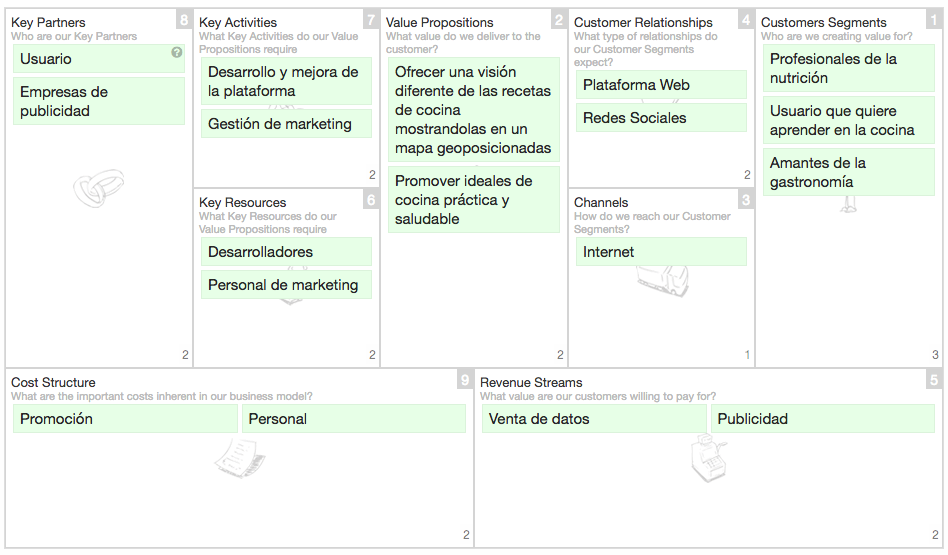
\includegraphics[width=1.0\textwidth]{imagenes/business-canvas.png}
\caption{Listado de elementos}
\label{business-canvas}
\end{center}
\end{figure}

Despues de desarrollar un producto mínimo viable de la aplicación de Njoycooking, se plantea la siguiente cuestión: ¿Es posible generar un modelo de negocio para la aplicación?

Mediante un business model canvas(figura \ref{business-canvas}) se describe de una forma simple en que consiste la idea de negocio.

\vspace{5 mm}

Al generar un modelo de negocio, el primer concepto que se tiene que valorar es: ¿Qué propuesta de valor ofrece la aplicación? es decir que elemento diferenciador puede ofrecer la aplicación frente otros existentes en el mercado. NjoyCooking es una aplicación gastronómica pero además de ofrecer un blog de cocina proporciona un visión diferente de los recetas de cocina, mostrando lo que cocina la gente según su zona geográfica mostrando las recetas geoposicionadas en un mapa y en tiempo real. Otra propuesta, es la de promover los hábitos de cocina práctica y saludable.


\vspace{5 mm}

Otro concepto que se tiene que valorar es como relacionarse con el cliente. El principal punto de contacto con los clientes será la aplicación web, donde los usuarios podrán interactuar y conocer la propuesta de valor que ofrece. Otra forma de contactar será mediante las redes sociales, ya que son un medio de difusión muy importante para a dar a conocer la aplicación.

\vspace{5 mm}

¿De dónde se obtendrán los ingresos? Las principales fuentes de ingresos serán dos:

\begin{description}

\item [Publicidad:] se proporcionará a las empresas la posibilidad de anunciarse en el sitio web mediante banners.

\item [Venta de datos]: los datos recogidos en la aplicación se ofrecerán a cambio de un pago económico a las empresas interesadas. Estos datos pueden servir a las empresas, que pueden realizar un estudio de mercado con ellos en función de las gustos y preferencias que tienen los usuarios de NjoyCooking.

\end{description}

\vspace{5 mm}

¿Cuáles son las fuentes clave? ¿Es decir que personal se necesita para llevar a cabo la propuesta de valor? Para cumplir la propuesta de valor se necesitará la contratación de programadores de software para desarrollar y mejorar la aplicación y especilistas en marketing para dar a conocer la aplicación y ofrecer un mejor uso y experiencia de ella.

\vspace{5 mm}

El usuario activo de la aplicación será el principal partner de la aplicación, ya que podrá promover la plataforma a sus conocidos y así abarcar un mayor número de usuarios. Las empresas de marketing y publicidad también se tienen en cuenta ya que pueden ayudar a llevar a cabo la propuesta de valor patrocinando el producto.


\vspace{5 mm}

Por último se debe tener en cuenta: ¿A qué público va enfocada la propuesta de valor? NjoyCooking tiene como objetivo un público concreto como son los amantes de la gastronomía y cocina en general. Aunque el objetivo es específico, engloba un abánico de usuarios amplio donde existe una variedad por edad,sexo,profesión o aptitudes culinarias.
